\documentclass[border=10pt]{standalone}

\usepackage{tikz}
\usepackage{tikzsymbols}
\usetikzlibrary{calc,patterns,shapes.geometric}

\def\centerarc[#1](#2)(#3:#4:#5){\draw[#1] ($(#2)+({#5*cos(#3)},{#5*sin(#3)})$) arc (#3:#4:#5);}

\begin{document}
	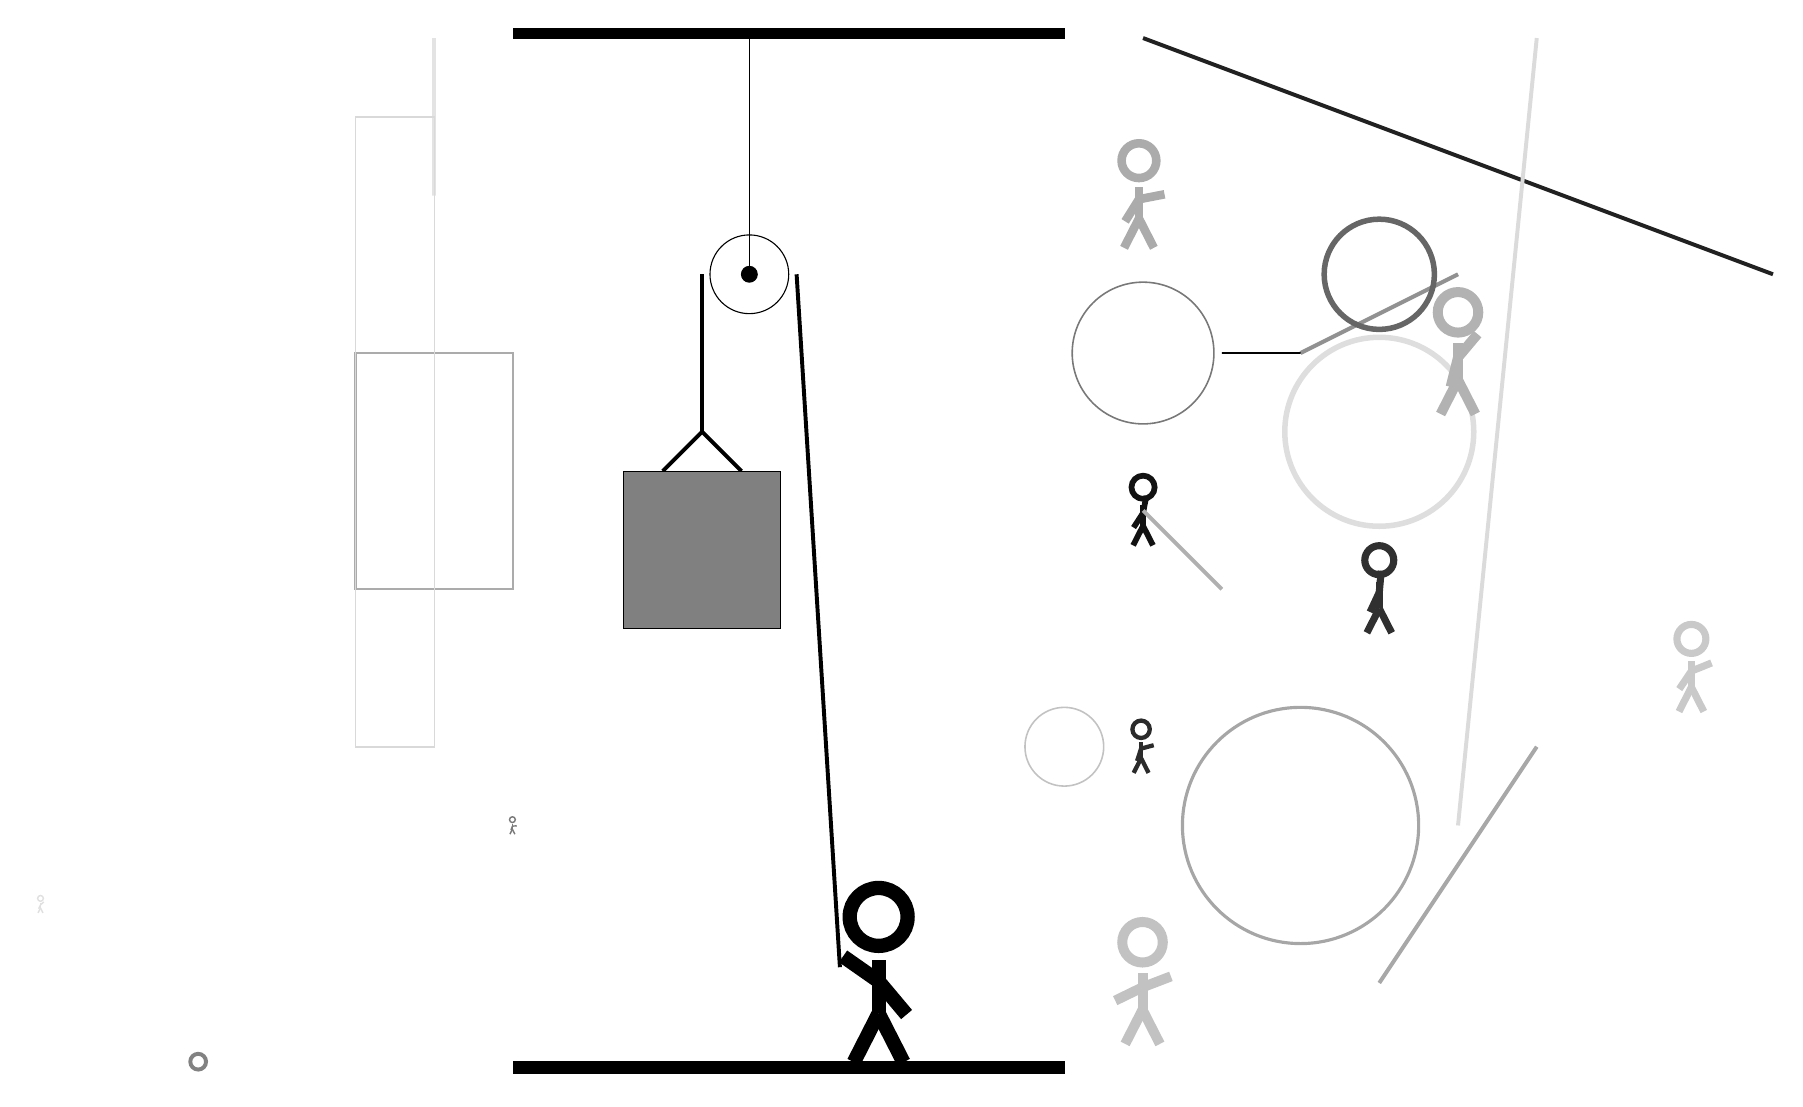
\begin{tikzpicture}
		%%%%% START %%%%%
		
		\draw[fill=black] (-2, 10) rectangle (5, 10.125);
		
		\draw (1, 7) circle (0.5);
		\draw[fill=black] (1, 7) circle (0.1);
		\draw (1, 10) -- (1, 7);
		
		\draw[line width=0.5mm] (-0.1, 4.5) -- (0.4, 5.0) -- (0.9, 4.5);
		\draw[fill=black!50] (-0.6, 4.5) rectangle (1.4, 2.5);
		
		\draw[line width=0.5mm] (0.4, 7) -- (0.4, 5.0);
		\centerarc[line width=0.5mm](1, 7)(0:180:0.6);
		\draw[line width=0.5mm](1.6, 7) -- (2.15, -1.8);
		
		\draw [line width=0.5mm, color=black!49](-6, -3) circle (0.1);
		
		\draw [line width=0.7mm, color=black!13](9, 5) circle (1.2);
		\node[line width=0.2mm, color=black!21] at (13, 2) {\Strichmaxerl[5][56][22]};
		\draw[line width=0.3mm, color=black!33] (-2, 3) rectangle (-4, 6);
		\draw[line width=0.5mm, color=black!11] (-3, 8) rectangle (-3, 10);
		\draw [line width=0.2mm, color=black!53](6, 6) circle (0.9);
		\node[line width=0.6mm, color=black!12] at (-8, -1) {\Strichmaxerl[1][64][41]};
		\draw[line width=0.5mm, color=black!34](9, -2) -- (11, 1);
		\node[line width=0.5mm, color=black!93] at (6, 4) {\Strichmaxerl[4][57][79]};
		\draw[line width=0.5mm, color=black!87](6, 10) -- (14, 7);
		\draw[line width=0.5mm, color=black!31](6, 4) -- (7, 3);
		\node[line width=0.6mm, color=black!24] at (6, -2) {\Strichmaxerl[7][26][21]};
		\node[line width=0.4mm, color=black!33] at (6, 8) {\Strichmaxerl[6][58][11]};
		\draw[line width=0.2mm, color=black!15] (-4, 1) rectangle (-3, 9);
		\draw[line width=0.5mm, color=black!43](10, 7) -- (8, 6);
		\draw[line width=0.2mm, color=black!99] (7, 6) rectangle (8, 6);
		
		\draw[line width=0.5mm, color=black!14](10, 0) -- (11, 10);
		\node[line width=0.5mm, color=black!52] at (-2, 0) {\Strichmaxerl[1][71][3]};
		\draw [line width=0.2mm, color=black!24](5, 1) circle (0.5);
		
		\draw [line width=0.4mm, color=black!35](8, 0) circle (1.5);
		\node[line width=0.6mm, color=black!83] at (6, 1) {\Strichmaxerl[3][72][15]};
		
		\draw [line width=0.7mm, color=black!60](9, 7) circle (0.7);
		
		\node[line width=0.4mm, color=black!81] at (9, 3) {\Strichmaxerl[5][65][85]};
		\node[line width=0.3mm, color=black!30] at (10, 6) {\Strichmaxerl[7][76][50]};
		
		\node at (2.6, -1.9) {\Strichmaxerl[10][-35][-50]};
		
		\draw[fill=black] (-2, -3) rectangle (5, -3.15);
		
		%%%%% END %%%%%
	\end{tikzpicture}
\end{document}